\chapter{Ausarbeitung}
\section{Aufgabe 1}
Die Residuen von L1 und L2 liegen in \autoref{fig:A1Residual}
\begin{figure}[ht]\centering 
	\subfigure[Residual L1]{
		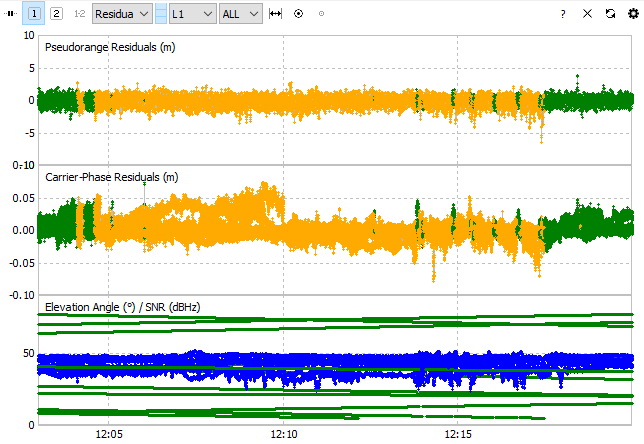
\includegraphics[width=0.5\textwidth]{A1ResidualL1.png}}
	\subfigure[Residual L2]{
		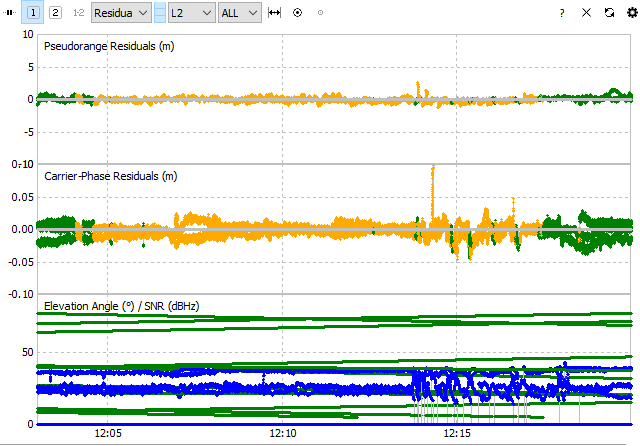
\includegraphics[width=0.5\textwidth]{A1ResidualL2.png}}
	\caption{Residuen}
	\label{fig:A1Residual}
\end{figure}
\clearpage
Die Ratio \autoref{fig:Ratio} und Standardabweichung \autoref{fig:A1std}
\begin{figure}[ht]\centering 
	\subfigure[Ratio]{
		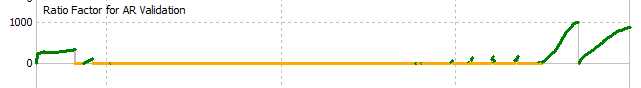
\includegraphics[width=0.8\textwidth]{A1Ratio.png}}
	\caption{Ratio}
	\label{fig:Ratio}
\end{figure}
\begin{figure}[ht]\centering 
	\subfigure[Position]{
		\includegraphics[width=0.45\textwidth]{A1pos.png}}
	\subfigure[Geschwindigkeit]{
		\includegraphics[width=0.45\textwidth]{A1vel.png}}
	\caption{Standardabweichungen}
	\label{fig:A1std}
\end{figure}\\
Auf diesen Parametern sind die Residuen relativ groß, in meisten Zeit sind die Ratio nicht ideal und die Standardabweichung sind währende einer Zeitdauer groß. \\\\
\clearpage
\section{Aufgabe 2}
\subsection{Mehr Beobachtungen}
Die Residuen \autoref{fig:A1Residualgalileo}, Ratio \autoref{fig:RatioGalileo} und Standardabweichung \autoref{fig:stdgal}, wenn man GPS und Galileo genutzt hat.
\begin{figure}[ht]\centering  
	\subfigure[Residual L1]{
	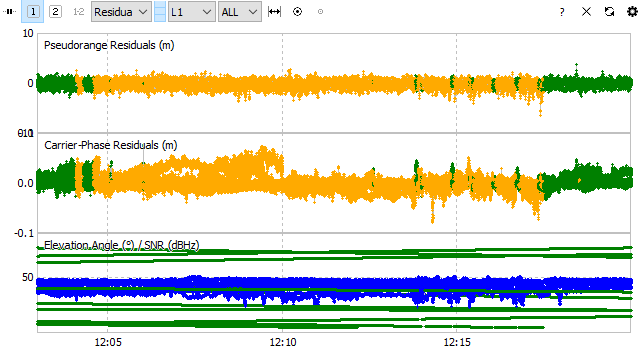
\includegraphics[width=0.5\textwidth]{A2GallileoResidualL1.png}}
\subfigure[Residual L2]{
	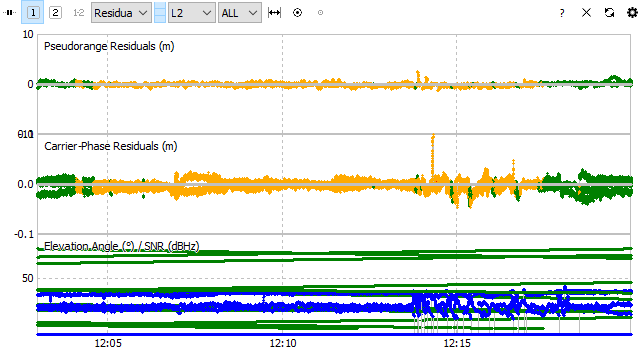
\includegraphics[width=0.5\textwidth]{A2GallileoResidualL2.png}}
\caption{Residuen}
\label{fig:A1Residualgalileo}
\end{figure}
\begin{figure}[ht]\centering 
	\subfigure[Ratio]{
		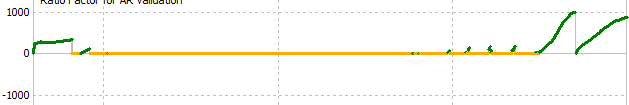
\includegraphics[width=0.8\textwidth]{A2GallileoRatio.png}}
	\caption{Ratio}
	\label{fig:RatioGalileo}
\end{figure}
\begin{figure}[ht]\centering 
	\subfigure[Position]{
		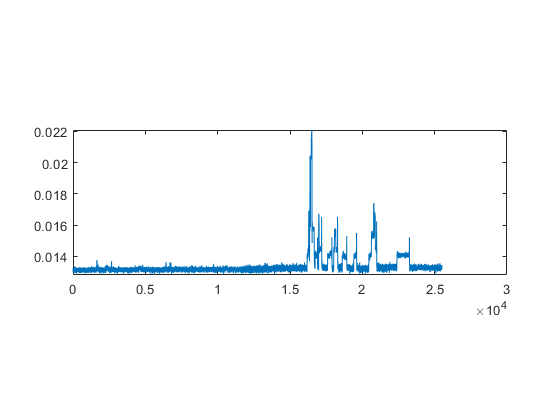
\includegraphics[width=0.45\textwidth]{galpos.png}}
	\subfigure[Geschwindigkeit]{
		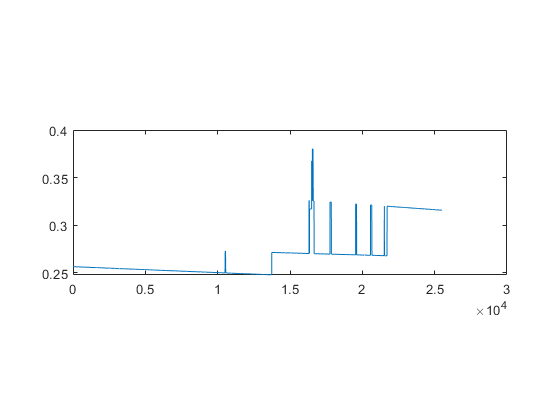
\includegraphics[width=0.45\textwidth]{galvel.png}}
	\caption{Standardabweichungen}
	\label{fig:stdgal}
\end{figure}\\
Es ist zu sehen, dass mehr Beobachtungen keinen sichtbare Verbesserung auf die Ergebnisse haben.
\newpage
\subsection{Elevationswinkel}
Minimaler Elevationswinkel werden bei dem Fall jeweils von $5^{\circ}$ erhöhen.\\\\
Die Residuen \autoref{fig:el10residuen}, Ratio \autoref{fig:el10residuen} und Standardabweichung \autoref{fig:stdel10} für Elevationsmaske $10^{\circ}$\\\\
Die Residuen \autoref{fig:el15residuen}, Ratio \autoref{fig:el15residuen} und Standardabweichung \autoref{fig:stdel15} für Elevationsmaske $15^{\circ}$
\begin{figure}[ht]\centering  
	\subfigure[Residual L1]{
		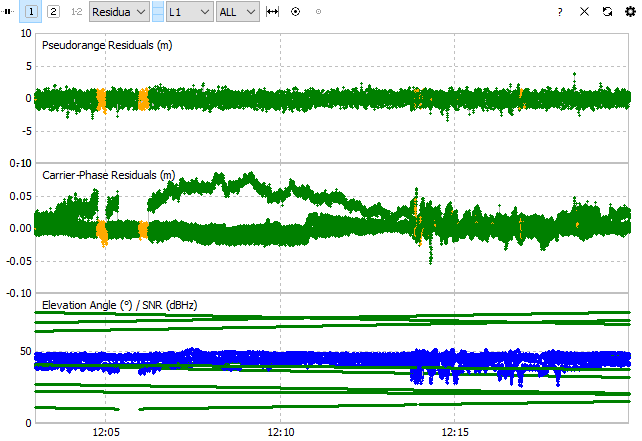
\includegraphics[width=0.5\textwidth]{A2el10L1.png}}
	\subfigure[Residual L2]{
		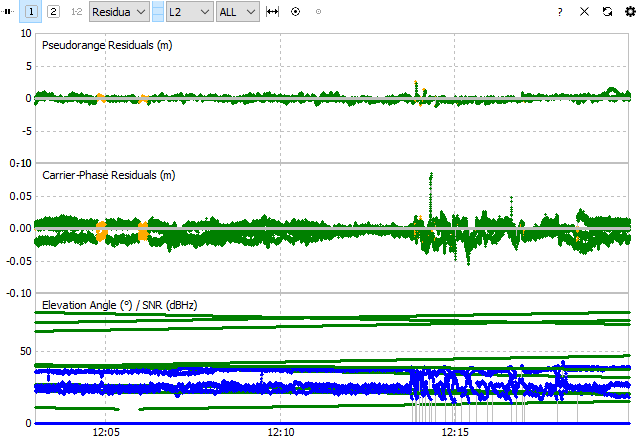
\includegraphics[width=0.5\textwidth]{A2el10L2.png}}
	\caption{Residuen Elevationsmaske $10^{\circ}$}
	\label{fig:el10residuen}
\end{figure}
\begin{figure}[ht]\centering 
	\subfigure[Ratio]{
		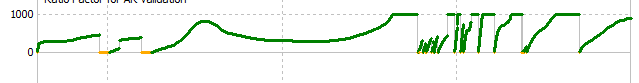
\includegraphics[width=0.8\textwidth]{A2Ratioel10.png}}
	\caption{Ratio Elevationsmaske $10^{\circ}$}
	\label{fig:Ratioel10}
\end{figure}
\begin{figure}[ht]\centering 
	\subfigure[Position]{
		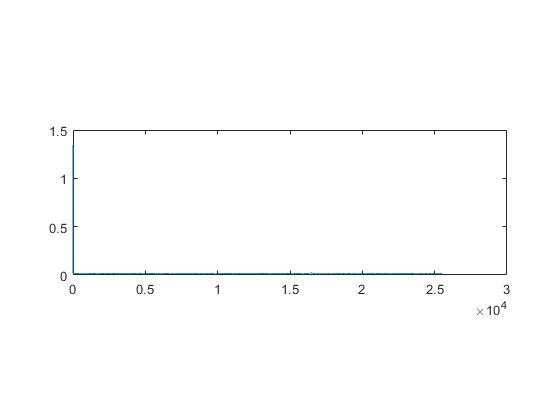
\includegraphics[width=0.45\textwidth]{el10pos.png}}
	\subfigure[Geschwindigkeit]{
		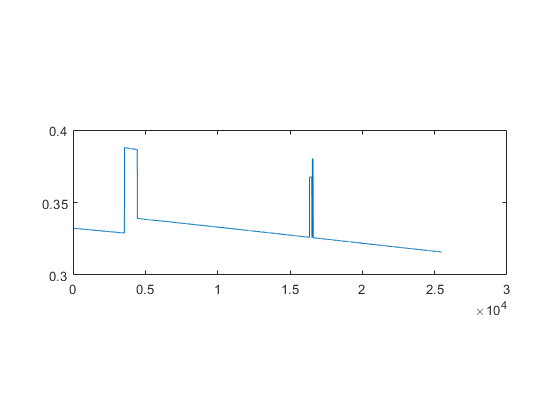
\includegraphics[width=0.45\textwidth]{el10vel.png}}
	\caption{Standardabweichungen Elevationsmaske $10^{\circ}$}
	\label{fig:stdel10}
\end{figure}
\begin{figure}[ht]\centering  
	\subfigure[Residual L1]{
		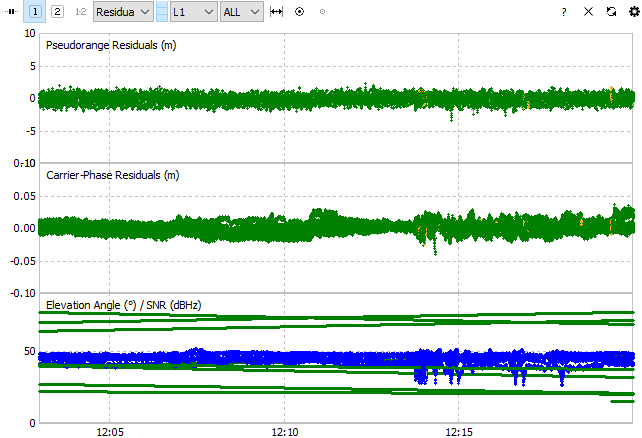
\includegraphics[width=0.5\textwidth]{A2el15L1.png}}
	\subfigure[Residual L2]{
		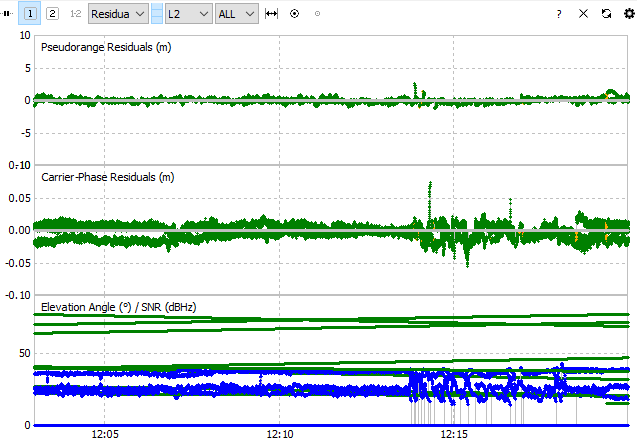
\includegraphics[width=0.5\textwidth]{A2el15L2.png}}
	\caption{Residuen Elevationsmaske $15^{\circ}$}
	\label{fig:el15residuen}
\end{figure}
\begin{figure}[ht]\centering 
	\subfigure[Ratio]{
		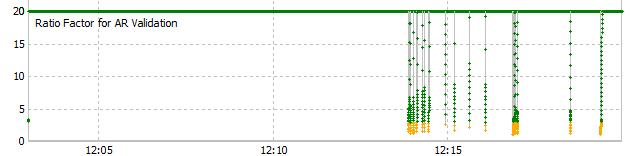
\includegraphics[width=0.8\textwidth]{A2Ratioel15.png}}
	\caption{Ratio Elevationsmaske $15^{\circ}$}
	\label{fig:Ratioel15}
\end{figure}
\begin{figure}[ht]\centering 
	\subfigure[Position]{
		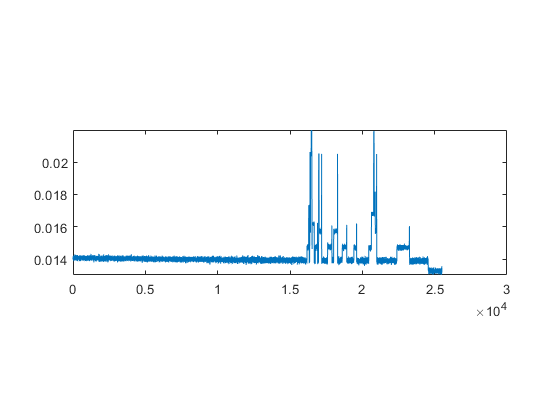
\includegraphics[width=0.45\textwidth]{el15pos.png}}
	\subfigure[Geschwindigkeit]{
		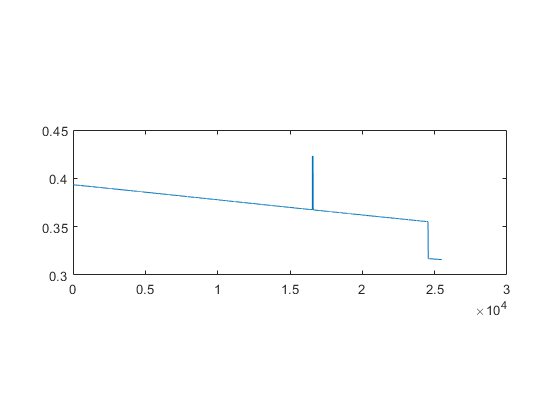
\includegraphics[width=0.45\textwidth]{el15vel.png}}
	\caption{Standardabweichungen Elevationsmaske $15^{\circ}$}
	\label{fig:stdel15}
\end{figure}\\\\
Wenn man die Elevationsmaske erhöhert, sind die Ergebnisse deutlich verbessert. 
\clearpage
\subsection{Kombinierte Lösung}
Eine kombinierte Lösung hat die Auswertung auch nicht verbessert. Die Residuen in \autoref{fig:residuenCombine}, Ratio in \autoref{fig:ratiocombine}, Standardabweichung in \autoref{fig:stdcombie}.
\begin{figure}[ht]\centering  
	\subfigure[Residual L1]{
		\includegraphics[width=0.5\textwidth]{CombieL1.png}}
	\subfigure[Residual L2]{
		\includegraphics[width=0.5\textwidth]{CombieL2.png}}
	\caption{Residuen kombinierte Lösung}
	\label{fig:residuenCombine}
\end{figure}
\begin{figure}[ht]\centering 
	\subfigure[Ratio]{
		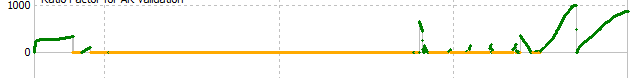
\includegraphics[width=0.8\textwidth]{ratiocombine.png}}
	\caption{Ratio kombinierte Lösung}
	\label{fig:ratiocombine}
\end{figure}
\clearpage
\begin{figure}[ht]\centering 
	\subfigure[Position]{
		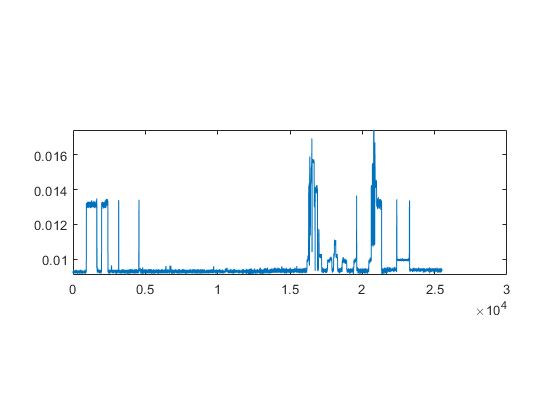
\includegraphics[width=0.45\textwidth]{combinepos.png}}
	\subfigure[Geschwindigkeit]{
		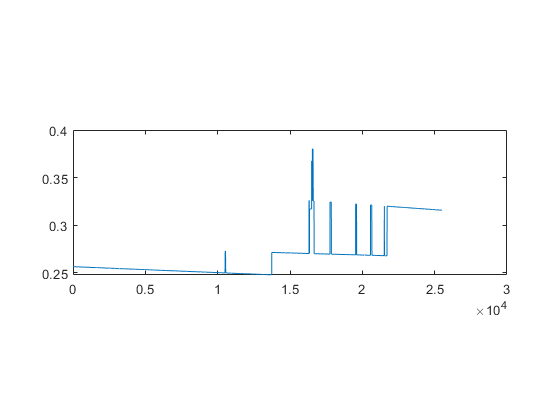
\includegraphics[width=0.45\textwidth]{combinevel.png}}
	\caption{Standardabweichungen kombinierte Lösung}
	\label{fig:stdcombie}
\end{figure}
Es ist zu sehen, dass 'cycle slip' eine wichtige Rolle bei Integer Ambiguity Fixierung spielen. Die Auswertung werden viel optimaler, wenn die Satelliten mit niedrige Elevationswinkel ausgefiltert werden. \clearpage
\section{Aufgabe 3}
In diesem Aufgabe werden ratio Schranke von in Schritte von 0.2 erniedrigt. Die Ergebnisse sind auch nicht viel geändert. Der Grund ist, der Ratio kann bis 1000 hoch sein. Wenn die Ratio von 3 von 0.2 reduziert ist, sind nur wenige nicht optimale Lösung ausgefiltert und die Verbesserung ist da nicht deutlich sichtbar.\\\\
\begin{figure}[ht]\centering  
	\subfigure[Residual L1]{
		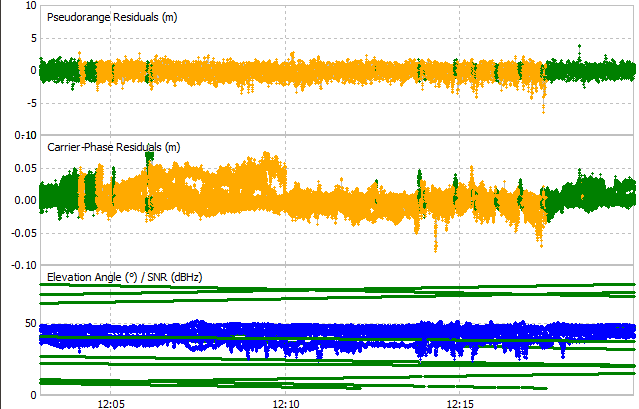
\includegraphics[width=0.5\textwidth]{28L1.png}}
	\subfigure[Residual L2]{
		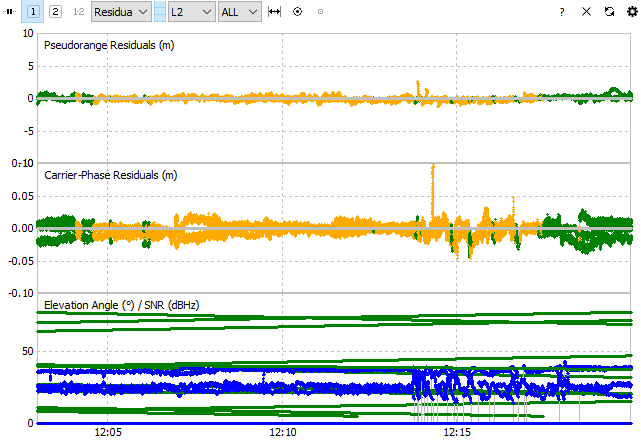
\includegraphics[width=0.5\textwidth]{28L2.png}}
	\caption{Residuen 2.8}
	\label{fig:resieuen28}
\end{figure}
\begin{figure}[ht]\centering 
	\subfigure[Ratio]{
		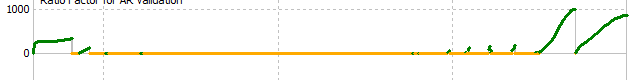
\includegraphics[width=0.8\textwidth]{26Ratio.png}}
	\caption{Ratio 2.8}
	\label{fig:ratio28}
\end{figure}
\begin{figure}[ht]\centering 
	\subfigure[Position]{
		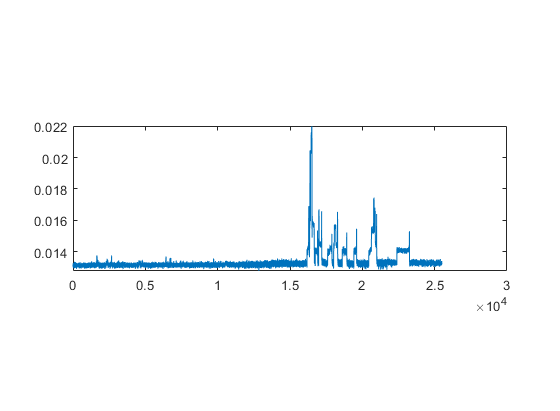
\includegraphics[width=0.45\textwidth]{28pos.png}}
	\subfigure[Geschwindigkeit]{
		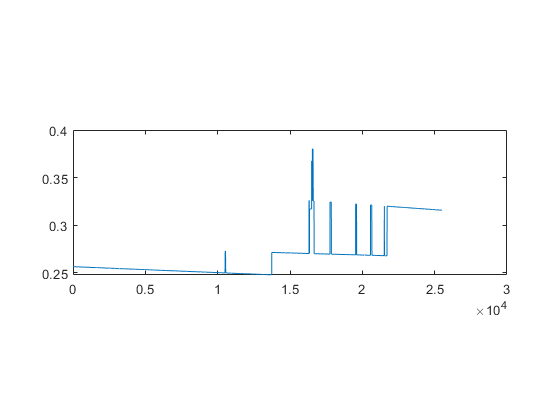
\includegraphics[width=0.45\textwidth]{28vel.png}}
	\caption{Standardabweichungen 2.8}
	\label{fig:std28}
\end{figure}
\begin{figure}[ht]\centering  
	\subfigure[Residual L1]{
		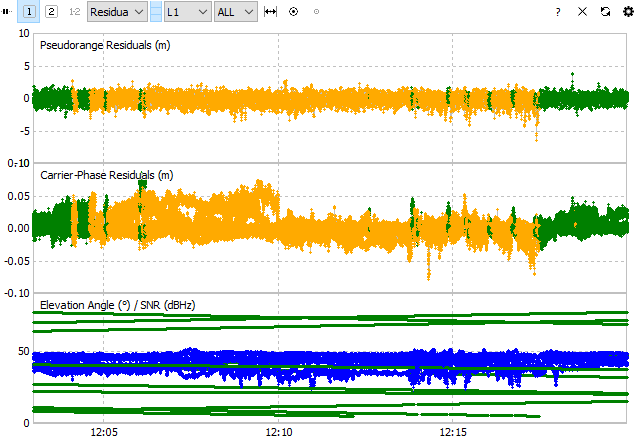
\includegraphics[width=0.5\textwidth]{26L1.png}}
	\subfigure[Residual L2]{
		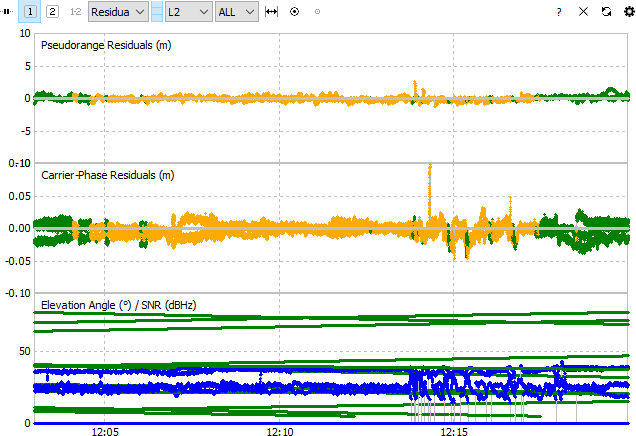
\includegraphics[width=0.5\textwidth]{26L2.png}}
	\caption{Residuen 2.6}
	\label{fig:resieuen26}
\end{figure}
\begin{figure}[ht]\centering 
	\subfigure[Ratio]{
		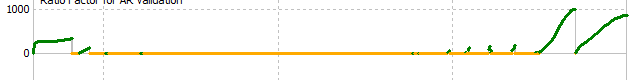
\includegraphics[width=0.8\textwidth]{26Ratio.png}}
	\caption{Ratio 2.6}
	\label{fig:ratio26}
\end{figure}
\begin{figure}[ht]\centering 
	\subfigure[Position]{
		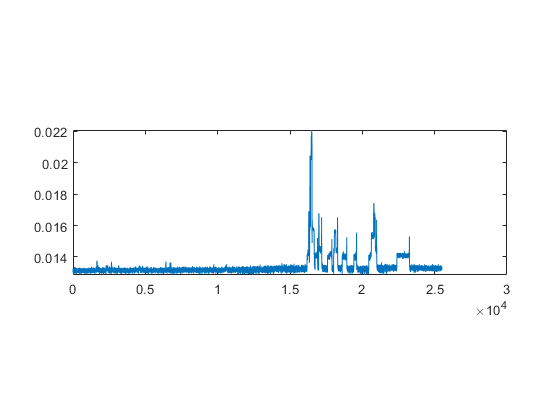
\includegraphics[width=0.45\textwidth]{26pos.png}}
	\subfigure[Geschwindigkeit]{
		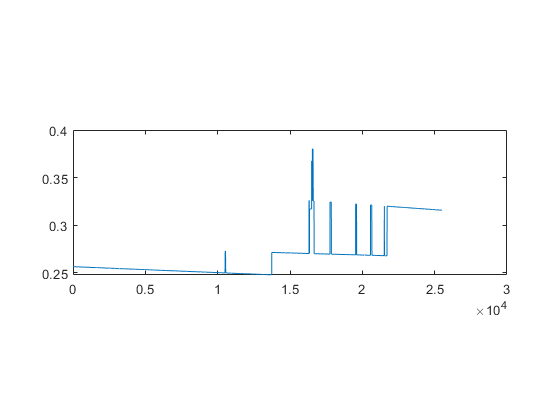
\includegraphics[width=0.45\textwidth]{26vel.png}}
	\caption{Standardabweichungen 2.6}
	\label{fig:std26111111}
\end{figure}